\chapter{Preface}
\section{Goals}
Before programming the robots, we must go over what we actually want to accomplish. Outside of simply "win autonomous routines, get WP, and have controls work," it is illustrative to list out more specific desires. For the software side of the robots, we are especially concerned with the following aspects (in order of precedence):
\begin{enumerate}
    \item Functionality
    \item Robustness
    \item Flexibility
\end{enumerate}

Functionality is, of course, principally important since, if the robot does not operate as intended by default, it does not matter what happens when a sensor fails or we need to quickly make a change. While those scenarios need to be considered, they do not score us points in-and-of themselves. Hence, functionality is the most important consideration. 

After that is robustness: what happens if $<$X$>$ fails? During Spin Up, in one autonomous routine at the World Championship the robot accidentally gathered more discs than allowed and we were disqualified; had we been able to detect such a scenario, we could have avoided that loss. In Over Under, in one autonomous routine at the World Championship, one of the motors on our intake arm went out and, because we had a PID controller managing the two sides being balanced using the motor encoders, the intake froze. Had we considered the possibility of one motor going out, the loss in that match could have been avoided. Therefore, we seek to develop a program that will respond to failures in a safe, reliable manner while notifying us of the problems that had occurred. 

Flexibility refers to the ability to trivially modify and add features to the software for the robot. Since scouting may reveal quirks in opponents autonomous routines, it would be helpful to be able to quickly add additional routines, for instance. Or, while testing, we may run into a new fail state that can be detected programmatically. Or, while testing, our drivers may discover that they do not feel comfortable with the current control scheme and may offer alternative suggestions. All-in-all, it is critical that our software is capable of undergoing rapid changes. 

\section{Principles}
\subsection{Work Process}
"Make it work. Make it right. Make it fast." \cite{bib:makeitworkmakeitright} is a maxim from Kent Beck that briefly summarizes our methodology when it comes to programming. The first task is to accomplish the basic goals we have in mind (make the drive move, get readings from encoders, etc.), make it work. After that, we should consider special cases and refactor to make the code clearer to understand, make it right. Lastly, if necessary, we should consider the performance of our code, make it fast. This process describes the majority of work on the software for the robots. 

We will typically immediately program for and test with real hardware. In some special circumstances, though, we may also incorporate additional planning before programming to the brain. Of course, there is always pencils and paper, but we may also incorporate the use of another tool or language like Python to prototype ideas. 

 "The Zen of Python" \cite{bib:pythonzen} more or less encapsulates the philosophy behind our work. Elegant solutions are of course preferred. Explicit statements are preferable to implicit statements, make good use of namespaces, make things readable, don't be a purist, so on and so on. 

\subsection{Style}
In order to support better readability, we make use of a consistent style throughout all files in the project. This is assisted via clang-format (which is discussed later) and auxiliary scripts to direct its use. 

\subsubsection{Names}
Names should of course be descriptive and brief, that should be a given. Additionally, we have a simple rule for the style of casing we use: pascal case (PascalCase) is used for classes, camel case (camelCase) is used for everything else. Even file names are written in camel case. 

\subsubsection{Assignment}
Any time we want to declare a variable, we have an order of precedence for mutability: 
\begin{enumerate}
    \item Constant expression
    \item Constant
    \item Mutable
\end{enumerate}
Constant expressions are essentially constants that can be determined at compile time. Constants, as the name implies, can not be modified after their initialization; whereas mutable items can be. We prefer constants over mutables to avoid incidental changes and be clear that said entity will not change. We prefer constant expressions over normal constants simply because of additional performance (constant expressions are not always possible in every situations, but nice when they are). 

\begin{lstlisting}[language=C++]
    constexpr int a{1}; // Constant expression
    const int b{2}; // Constant
    int c{3}; // Mutable
\end{lstlisting}

You will also note the use of curly braces to initialize values. This method is preferred over equal signs, because it will produce an error if implicit casting occurs. This ensures that casting from one type to another will only happen if done explicitly.  

Even methods associated with objects can be considered "constant," implying that calling the method will result in no change to the internal state of the object. 

\begin{lstlisting}[language=C++]
    class SomeClass {
    public:
        void constDemo() const;
    };

    void SomeClass::constDemo() const { ... }
\end{lstlisting}

\subsubsection{Comments}
There are two main types of comments: documentation and implementation. 

Documentation comments can be found in the header files for the project, and should be seen above every publicly-accessible entity. For our purposes (and in connection with Doxygen, which is discussed later) we use Javadoc-style comments \cite{bib:javadoc}. 

On the other hand, implementation comments should be relatively sparse, reserved for such scenarios where there is a reason the code can not simply be made made more clear in intent. 

This is an example of a documentation comment: 
\begin{lstlisting}[language=C++]
    /**
    * @brief A function made with the express purpose of 
    * visualizing how we employ comments in code.
    *
    */
    void commentDemo();
\end{lstlisting}

This is an example of an implementation comment (probably a pedantic one, though):
\begin{lstlisting}[language=C++]
    void commentDemo() {
        // The following notation supports breaking the returned pair into two values.  
        auto [v, a] = physicsMath();
        ...
    }
\end{lstlisting}

\subsubsection{References, Pointers, and Values}
Simply put, there are three main ways to pass a parameter into a procedure. The most straightforward is to pass by value, where the data is copied over into the respective parameter variables. This is okay for simpler structures like integers, floating-point values, and so on, but for larger structures like vectors this may entail a great deal of copying. 

In such cases, it may be preferable to pass the \textit{location} of the vector rather than copy over all the values, since the location is represented with a simple numeric value for its address. At which point, there are two options: references and pointers. 

References are similar to pointers but can not take on a null value and do not require the same de-referencing syntax. The later property was actually the reason references were created in the first place. See the following code \cite{bib:cppfaqstroustrup} from Bjarne Stroustrup, creator of C++:
\begin{lstlisting}[language=C++]
    void f1(const complex* x, const complex* y)	// without references
	{
		complex z = *x+*y;	// ugly
		// ...
	}

	void f2(const complex& x, const complex& y)	// with references
	{
		complex z = x+y;	// better
		// ...
	}
\end{lstlisting}

You will notice the use of constant here, since mutable references allow functions to change the passed in variable directly, which can be confusing. 

Pointers are typically associated with objects stored on dynamic, heap-allocated memory. The traditional method of allocating such space is the use of the new keyword followed (at some point) by de-allocation using delete. This is dangerous, since if the delete keyword is forgotten you have allocated memory that is never freed: a memory leak. Since dynamic allocation is incredibly common, this is a serious issue. Hence, introducing the use of smart pointers. 

Smart pointers are essentially wrappers around raw pointers to support implicit de-allocation. This is done with the idea of ownership: that these smart pointers "own" a resource. If no smart pointers own a resource it is deallocated (this is done by employing the destructor of the smart pointers, hence a smart pointer going out of scope releases its ownership). 

There are two (main) types of smart pointers: shared pointers and unique pointers. Shared pointers allow several shared pointers to own a resource. When one of these goes out of scope and its destructor called, the number of "owners" is decremented. When it reaches zero, the resource is deallocated. Unique pointers allow only one pointer to have ownership over the resource at any given time. If you want to transfer ownership, you have to explicitly do so using the move function. Raw pointers are still okay, though, so long as they are not responsible for allocating or deallocating memory (i.e., if they don't own the resource).

To summarize our use of pointers, references, and values, consider the diagram in \ref{fig:refpointvals}.
\begin{figure}
    \centering
    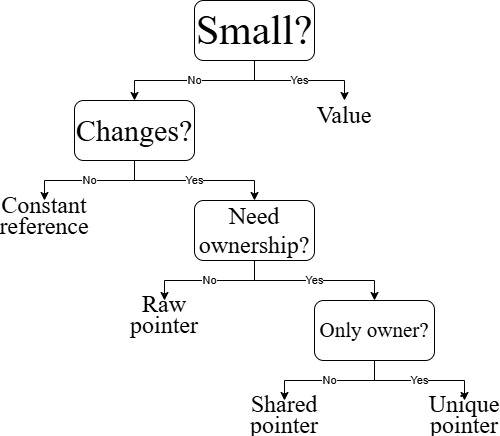
\includegraphics[width=0.75\linewidth]{images/software/preface/refpointval.jpg}
    \caption{What to use?}
    \label{fig:refpointvals}
\end{figure}

\subsubsection{Miscellaneous}
We prefer to make scope explicit to avoid common mistakes, that is to say we prefer
\begin{lstlisting}[language=C++]
    if(someCondition()) {
        doSomething();
    }
\end{lstlisting}
over
\begin{lstlisting}[language=C++]
    if(someCondition())
        doSomething();
\end{lstlisting}

We also prefer to place curly braces inline (though this is purely aesthetic), that is to say we prefer
\begin{lstlisting}[language=C++]
    void doSomething() {
    ...
    }
\end{lstlisting}
over
\begin{lstlisting}[language=C++]
    void doSomething() 
    {
    ...
    }
\end{lstlisting}

We place all code inside the atum namespace to avoid conflicts with similarly named entities in the standard library, PROS API, and so on. 

When we make use of templates, we tend to use aliases for the common parametrizations for the sake of readability.

\section{Tools}
In order to improve the development experience, we employ a multitude of software tools to support our programming efforts. Some of these are essential to our team, while others simply provide quality of life during coding.

\subsection{PROS}
We use PROS \cite{bib:pros} as our development platform for the robots. We could provide a design matrix of some sort for why we made this decision, but it's quite straightforward. 

There are pretty much three options:
\begin{itemize}
    \item PROS
    \item VEXcode
    \item Vexide
\end{itemize}

In the past there was also Robot Mesh Studio, but they are no longer continuing development. 

The differences between PROS and VEXcode at this point are quite mute, with the exception of the team's extensive experience using PROS. Historically, we preferred PROS over alternatives because of the freedom in what text editor we could use as well as the quality documentation and support (this was all in comparison to VEX Coding Studio). VEXcode at this point has similar documentation and support to PROS, especially with the recent update to PROS 4. Vexide, on the other hand, represents a stark departure from PROS and VEXcode, supporting Rust development. This is intriguing, but Vexide is early in development and perhaps illegal for competition use \cite{bib:vexidelegal}. 

One significant advantage PROS still has over VEXcode is that it is open source: so when we have a particularly strange issue, we can verify if it is an issue on our part or not. But, for the most part, they are quite comparable platforms. Again, the main reason we use PROS is our experience with the software.

\subsection{VSCode}
Visual Studio Code is our text editor of choice for writing programs. This is because Visual Studio Code strikes a decent balance between customization, power, and ease-of-use. 

VSCode also allows for the easy installation of extensions. Outside of common extensions for C++ development, we currently employ a few other extensions specifically for robotics software development: 
\begin{itemize}
    \item \href{https://github.com/purduesigbots/pros-vsc}{PROS-VSC}: for obvious reasons. 
    \item \href{https://github.com/cschlosser/doxdocgen}{Generate Doxygen Comments in VSCode}: provides a keyboard shortcut to produce a \textit{template} for methods, functions, and classes based on their parameters and return types, in accordance with Javadoc style comments. 
    \item \href{https://github.com/streetsidesoftware/vscode-spell-checker}{Spelling Checker for Visual Studio Code}: acts a spell checker even with camel case and pascal case. 
\end{itemize}

\subsection{Doxygen}
We use Doxygen \cite{bib:doxygen} to generate HTML from the Javadoc-style comments that we place throughout our header files. We also make use of Doxygen Awesome \cite{bib:doxygenawesome} to further stylize our documentation. This is useful (not only for notebook purposes) to provide additional resources for newer programmer on the team. 

Any judges can access our documentation \href{https://the-atu-robotics-club.github.io/ATUM-V5RC-High-Stakes-Code/index.html}{here}: \hspace{30px}
\qrcode[height = .3\linewidth]{https://the-atu-robotics-club.github.io/ATUM-V5RC-High-Stakes-Code/index.html}

If the links above are inaccesible, \ref{fig:web-docs-example} has a photo of one page of the documentation. 

\begin{figure}
    \centering
    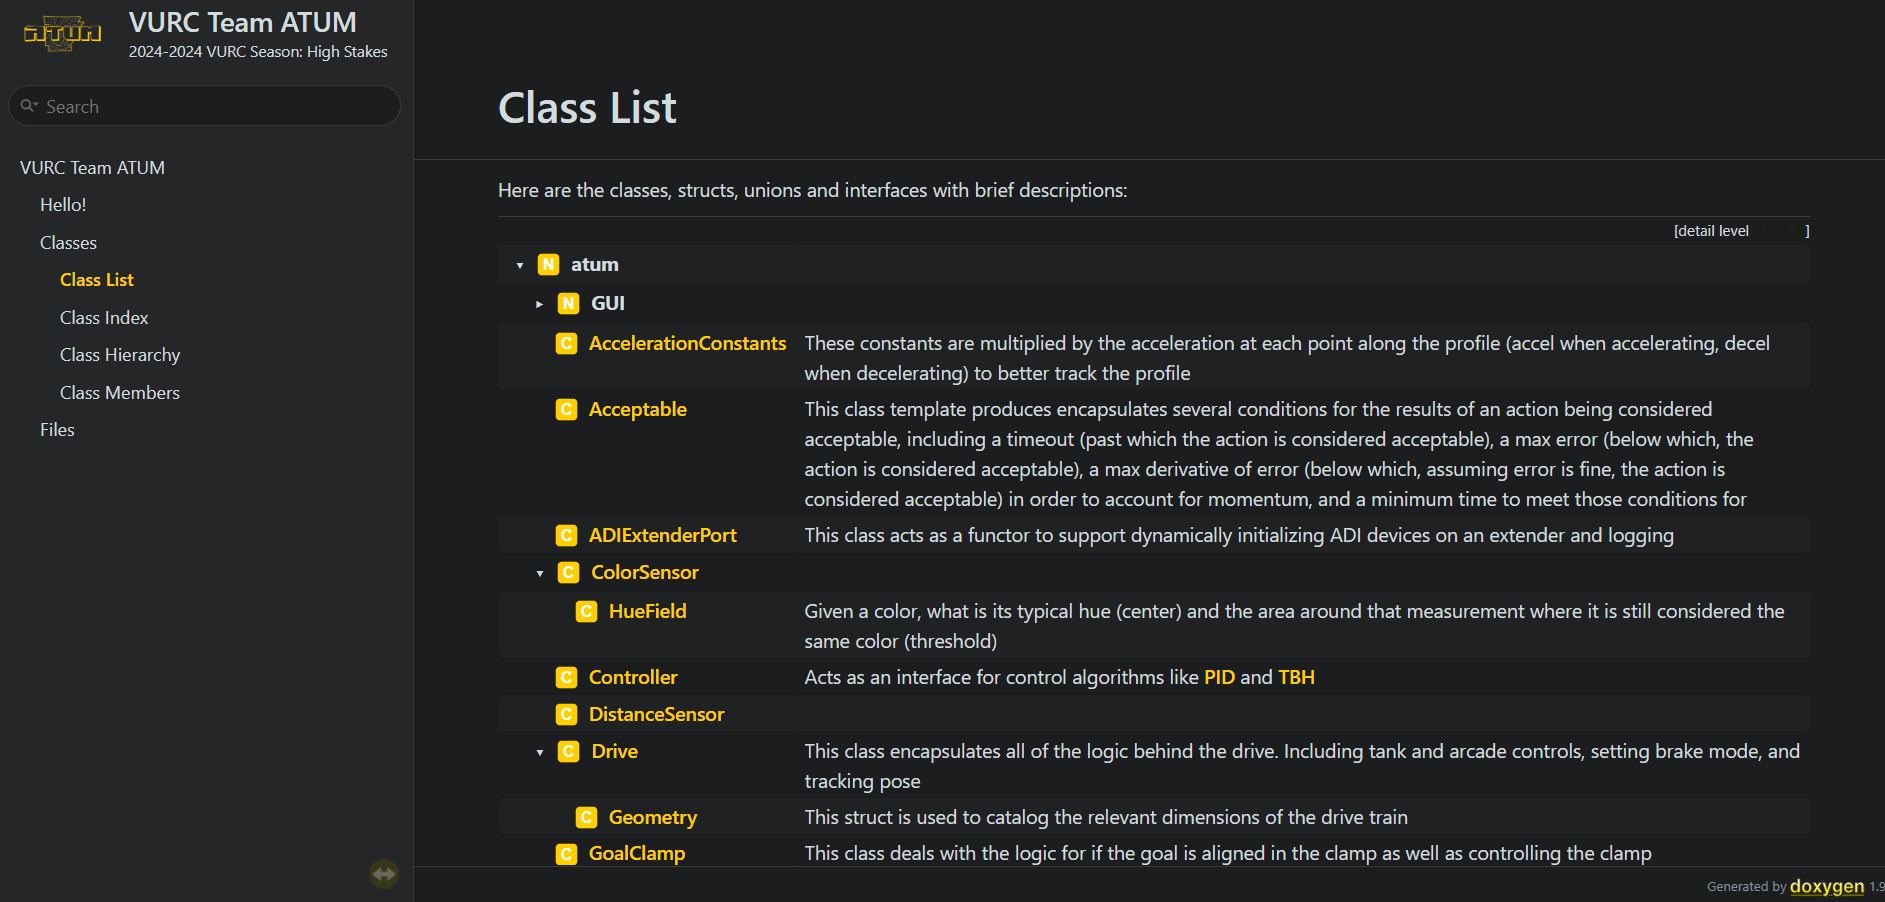
\includegraphics[width=0.75\linewidth]{images/software/preface/documentation webpage.png}
    \caption{The class list on our documentation page.}
    \label{fig:web-docs-example}
\end{figure}

\subsection{Libraries}
While we prefer to provide our own software solutions to whatever problems we face, occasionally a task would require a significant effort (several months/years) and would have little relevance to the actual behavior of the robot. In these circumstances, we make use of third-party libraries. 

\subsubsection{UNITS}
To support dimensional units (like meters, seconds, and so on), we employ the nholthaus UNITS library \cite{bib:nholthaus}. We went with this library, since it is header-only and therefore easy to set up. As a bonus, it is compile-time and efficient. 

The use of dimensional units represents a significant improvement in both ease-of-development, clarity of intent, and robustness. While the former two are easy to gather, it is not immediately clear how dimensional units prevent errors. Simply put, unit conversions are consistently performed throughout the project without conscious effort. While we could be careful to avoid, say, passing in a value we intend to be in radians to a function that expects degrees, it is nice to not have to worry at all. It sounds silly, but this exact problem has occurred for folks at NASA, with expensive consequences \cite{bib:marsclimateorbiter}.

\subsubsection{LVGL}
For developing the GUI for the brain screen, we employ LVGL (Light and Versatile Graphics Library) \cite{bib:lvgl}. We make use of LVGL because of ready prepared PROS templates to integrate the library into PROS projects. 

\subsection{Miscellaneous}
\subsubsection{GitHub}
Because we have covered GitHub earlier, we will be brief. We use git/GitHub not only for version control and project management, but also for the use of GitHub Actions and documentation hosting. 

GitHub actions allow us to employ GitHub's servers to perform certain actions upon pushing code, or upon request. We make use of this to keep our documentation up-to-date (by running Doxygen and updating the GitHub webpage) as well as formatting code using clang-format.

As implied, we also use GitHub for hosting our documentation. 

\subsubsection{clang-format}
Clang-format \cite{bib:clangformat} is used for automatically formatting our code based on a list of specifications. We also employ a console script to apply formatting to all files in the project (this script is ran by the formerly mentioned GitHub action upon request). 

\subsubsection{cppcheck}
Cppcheck \cite{bib:cppcheck} is used for static analysis of our code. This essentially provides additional checks over the program to detect issues that can not typically be caught by the compiler. 